\documentclass[11pt, oneside]{article}   	% use "amsart" instead of "article" for AMSLaTeX format
\usepackage{geometry}                		% See geometry.pdf to learn the layout options. There are lots.
\geometry{letterpaper}                   		% ... or a4paper or a5paper or ... 
\usepackage{graphicx}				% Use pdf, png, jpg, or eps§ with pdflatex; use eps in DVI mode
								% TeX will automatically convert eps --> pdf in pdflatex		
\usepackage{amssymb}
\usepackage{program}

\title{Assignment 4: Decision Making under Uncertainty and Learning}
\author{Alex Smirnov, Scott Reyes}
\date{May 1, 2017}							

\begin{document}
\maketitle
%\section{}
%\subsection{}
\begin{flushleft}

\section*{Question 1:}

\section*{Question 2:}
\subsection*{a}

\subsection*{b}

\subsection*{c}

\section*{Question 3:}
\subsection*{a}

\subsection*{b}

\subsection*{c}

\section*{Question 4:}
\subsection*{a}
Constant offset = 1\\
Class -1 Inputs:\\
(0.1, 1), (0.35, 0.95), (0.7, 0.65), (0.9, 0.45)\\
Class 1 Inputs: \\
(0.1, 0.7), (0.3, 0.55), (0.45, 0.15), (0.6, 0.3)\\
Initial Weights:\\
$w_0 = 0.2$\\
$w_1 = 1$\\
$w_2 = -1$\\
$y=(0.2*1)+((0.1*-1)+(0.35*-0.95)+(0.7*-0.65)+(0.9*-0.45)+(0.1*-0.7)+(0.3*-0.55)+(0.45*-0.15)+(0.6*-0.3))x$\\
$y=0.2+(-0.1-0.3325-0.455-0.405-0.07-0.165-0.0675-0.18)x$\\
$y=-1.775x+0.2$\\
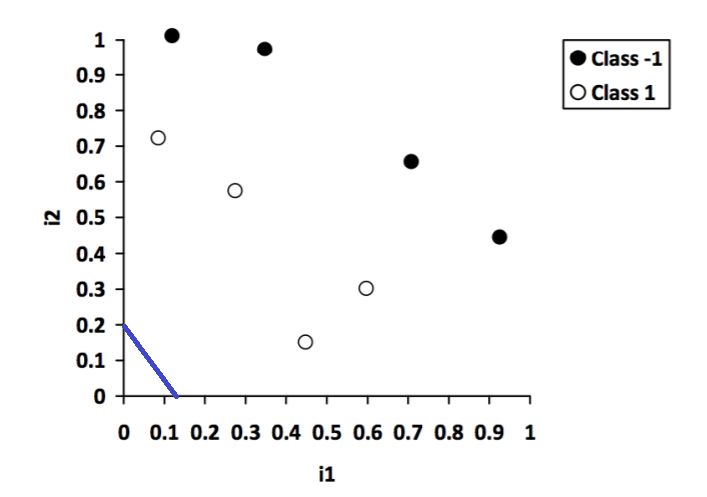
\includegraphics[]{q4_1.png}
\\
4 samples are misclassified after the initial line of separation is placed. Class 1 input (0.1, 0.7) is misclassified, so the weights will be adjusted accordingly.\\
$w_0 = 1$\\
$w_1 = 1$\\
$w_2 = -1$\\
$y=(1*1)+((0.1*-1)+(0.35*-0.95)+(0.7*-0.65)+(0.9*-0.45)+(0.1*-0.7)+(0.3*-0.55)+(0.45*-0.15)+(0.6*-0.3))x$\\
$y=1+(-0.1-0.3325-0.455-0.405-0.07-0.165-0.0675-0.18)x$\\
$y=-1.775x+1$\\
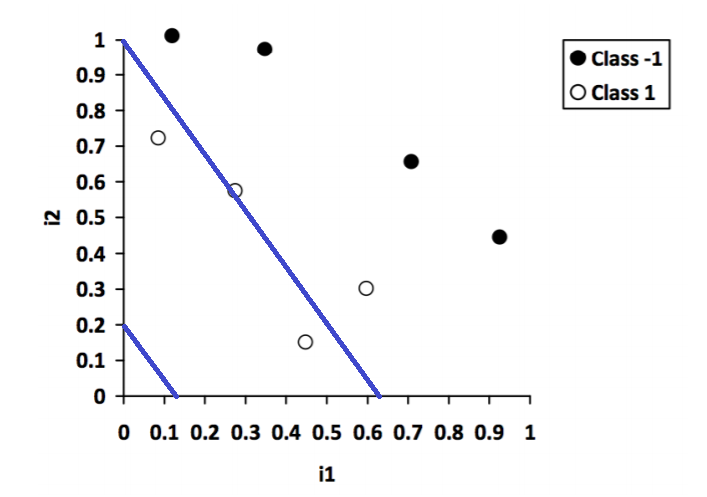
\includegraphics[]{q4_2.png}
\\
2 samples are misclassified after the second line is placed. Class 1 input (0.3, 0.55) is misclassified, so the weights will be adjusted accordingly.\\
$w_0 = 1$\\
$w_1 = 0.8$\\
$w_2 = -1$\\
$y=(1*1)+((0.08*-1)+(0.28*-0.95)+(0.56*-0.65)+(0.72*-0.45)+(0.08*-0.7)+(0.24*-0.55)+(0.36*-0.15)+(0.48*-0.3))x$\\
$y=1+(-0.08-0.266-0.364-0.324-0.056-0.132-0.054-0.144)x$\\
$y=-1.42x+1$\\
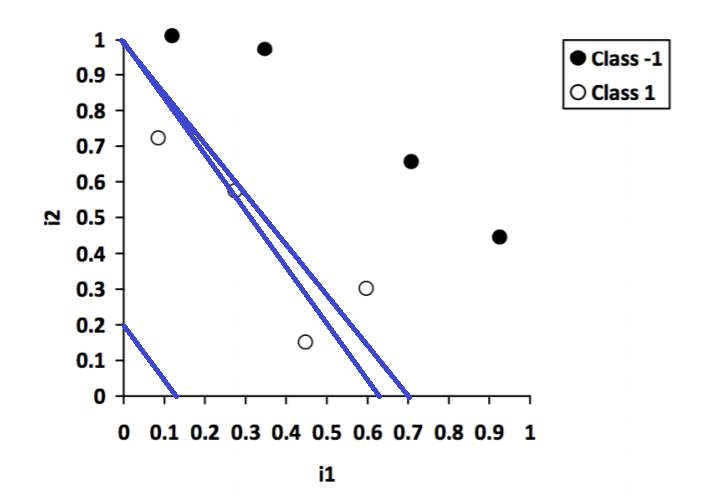
\includegraphics[]{q4_3.png}
\\
1 sample is misclassified after the third line is placed. Class 1 input (0.6, 0.3) is misclassified, so the weights will be adjusted accordingly.\\
$w_0 = 1$\\
$w_1 = 0.5$\\
$w_2 = -1$\\
$y=(1*1)+((0.05*-1)+(0.175*-0.95)+(0.35*-0.65)+(0.45*-0.45)+(0.05*-0.7)+(0.15*-0.55)+(0.225*-0.15)+(0.3*-0.3))x$\\
$y=1+(-0.05-0.16625-0.2275-0.2025-0.035-0.0825-0.03375-0.09)x$\\
$y=-0.8875x+1$\\
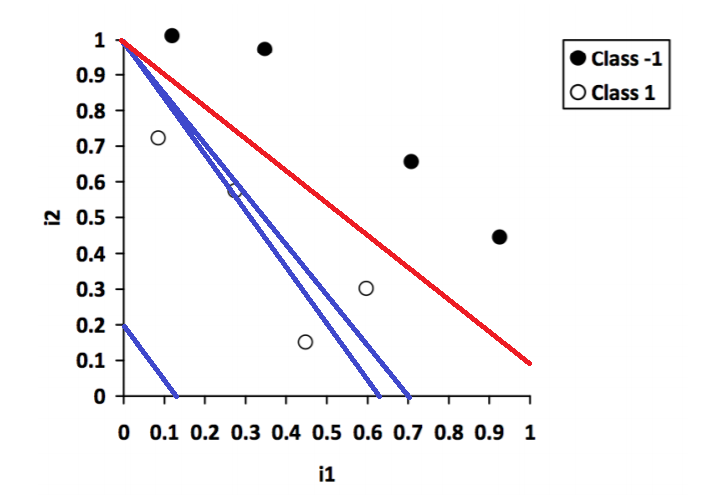
\includegraphics[]{q4_4.png}
No samples are misclassified after the fourth line is placed.\\
\subsection*{b}
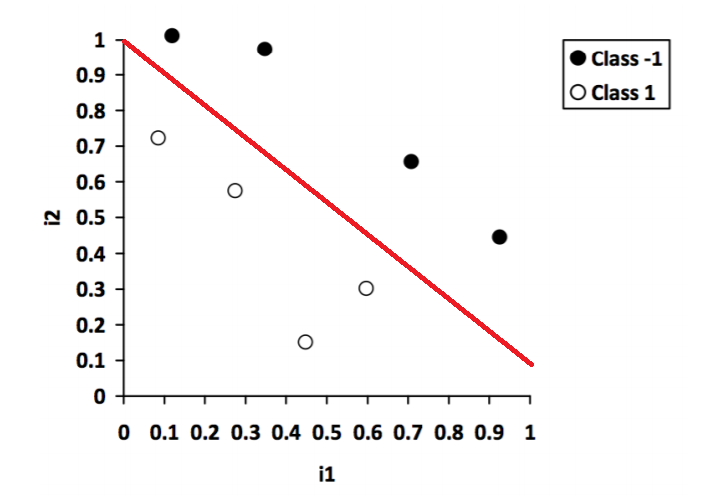
\includegraphics[]{q4_final.png}
\\
This is the final line that achieved perfect classification.\\
$w_0 = 1$\\
$w_1 = 0.5$\\
$w_2 = -1$\\
$y=-0.8875x+1$\\
\subsection*{c}
Constant offset = 1\\
Class -1 Inputs:\\
(0.1), (0.35), (0.7), (0.9)\\
Class 1 Inputs: \\
(0.1), (0.3), (0.45), (0.6)\\
Initial Weights:\\
$w_0 = 1$\\
$w_1 = -0.25$\\
$y=(1*1)+(-0.025-0.0875-0.175-0.225-0.025-0.075-0.1125-0.15)x$\\
$y=-0.875+1$\\
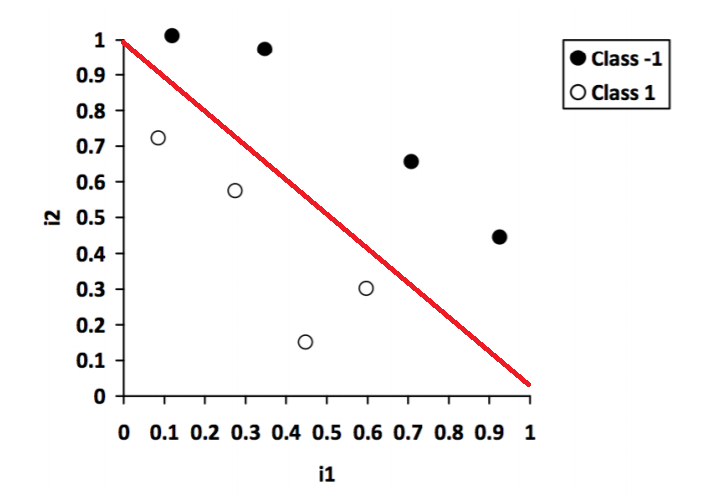
\includegraphics[]{q4_c_final.png}
\\
The error for this input space separation is 0 because all of the inputs are correctly classified.\\
\section*{Question 5:}
\subsection*{a}
The minimum error that can be reached with a single perceptron for this classification task is 2, which means 2 points will be classified incorrectly no matter how much learning the perceptron does.\\
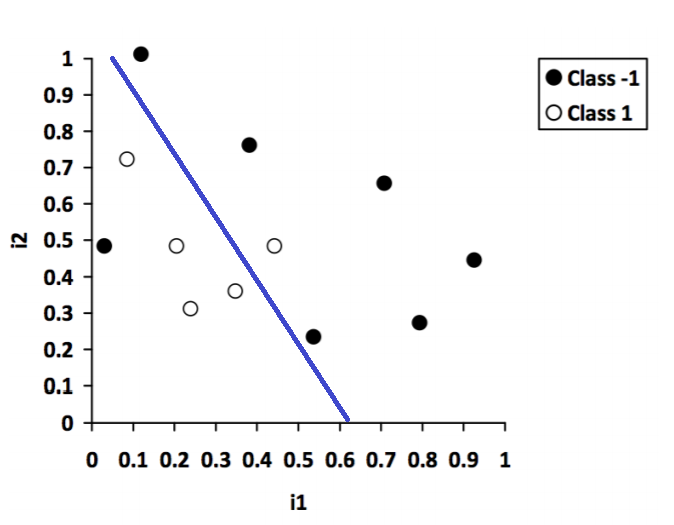
\includegraphics[]{q5_line_1.png} \\
\subsection*{b}
Final result of the multilayer perceptron line drawing: \\
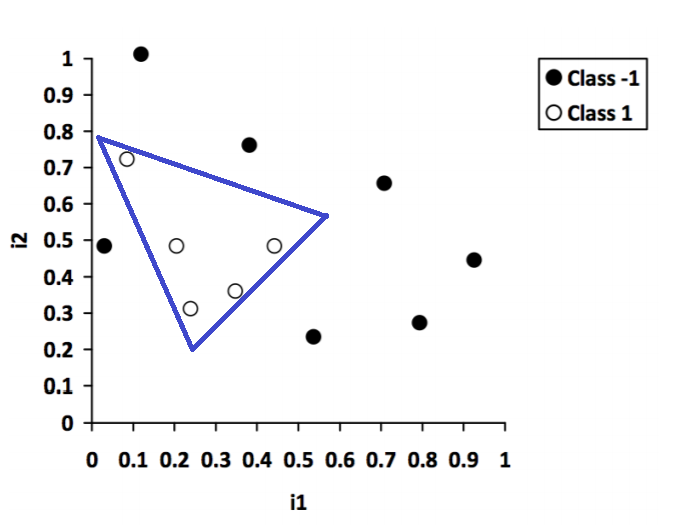
\includegraphics[]{q5_mlp.png}
%need to finish multilayer perceptron network

\end{flushleft}
\end{document}  